\chapter{МЕТОДЫ УПРАВЛЕНИЯ ЭЛЕКТРОПНЕВМАТИЧЕСКИМ ПРИВОДОМ С ДИСКРЕТНЫМ УПРАВЛЕНИЕМ}\label{ch:ch3}
Управление электропневматическими приводами с дискретными распределителями представляет
собой комплексную задачу, обусловленную нелинейной динамикой пневматических систем и
дискретным характером управляющих воздействий. Эффективное решение данной задачи требует
применения специализированных алгоритмов, способных обеспечить высокую точность позиционирования и
быстродействие системы при ограниченном наборе управляющих состояний. Особый интерес представляет адаптация
классических методов управления к специфике дискретных пневматических систем.

В рамках настоящего исследования рассматривается широкий спектр подходов к управлению электропневматическими
приводами, включающий как современные адаптивные методы, так и модифицированные
классические алгоритмы. Исследуются скользящее управление, прогнозное управление,
нечеткое управление, нейросетевое управление, а также применение широтно-импульсной модуляции (ШИМ)
в сочетании с классическими регуляторами, такими как ПИД-регулятор и его модификации.
Выбор данных методов обусловлен необходимостью комплексного анализа возможностей оптимизации управления
с учетом специфики дискретных пневматических систем. Каждый из рассматриваемых подходов обладает
уникальными преимуществами и ограничениями, детальное изучение которых позволит сформировать
всестороннее представление о перспективах совершенствования алгоритмов управления
электропневматическими приводами с дискретными распределителями.

\section{Анализ режимов работы электропневмопривода}\label{sec:ch3/sec1}

Функционирование электропневмопривода с дискретными распределителями характеризуется конечным
множеством возможных состояний системы, определяемых комбинациями состояний распределителей.
Математически пространство состояний распределителей может быть представлено как:

\begin{equation}\label{eq:state_space}
	\mathbf{U} = \left\{
	[u_1, u_2, u_3, u_4] | u_i \in {0,1}, i = 1,\dots,4
	\right\},
\end{equation}
где $u_i$ -- состояние i-го распределителя (0 - закрыт, 1 - открыт).

Теоретически система, как описано ранее, допускает $2^4 = 16$ различных комбинаций состояний распределителей.
Однако с учетом физических ограничений и требований безопасности целесообразно использование только определенного
подмножества состояний, формирующих основные режимы работы привода.

Классификация этих режимов представлена в следующей таблице \ref{tab:operation_modes}.

\begin{table}[htbp]
	\centering
	\caption{Режимы работы электропневматического привода с дискретными распределителями}
	\label{tab:operation_modes}
	\small
	\begin{tabular}{lcll}
		\midrule
		\textbf{Режим}             & $[u_1,u_2,u_3,u_4]$ & \textbf{Движение} & \textbf{Динамика} \\
		\midrule
		С.П.У.\textsuperscript{1}  & $[1,0,0,1]$         &
		Макс. положит. ускорение   &
		$M\ddot{x} = p_\text{п}F_1 - p_\text{атм}F_2 - R_\text{тр}$                              \\

		У.П.У.\textsuperscript{2}  & $[1,0,0,0]$         &
		Умер. положит. ускорение   &
		$M\ddot{x} = p_\text{п}F_1 - p_2F_2 - R_\text{тр}$                                       \\

		Сл.П.У.\textsuperscript{3} & $[0,0,0,1]$         &
		Мин. положит. ускорение    &
		$M\ddot{x} = p_1F_1 - p_\text{атм}F_2 - R_\text{тр}$                                     \\

		С.О.У.\textsuperscript{4}  & $[0,1,1,0]$         &
		Макс. отриц. ускорение     &
		$M\ddot{x} = p_\text{атм}F_1 - p_\text{п}F_2 - R_\text{тр}$                              \\

		У.О.У.\textsuperscript{5}  & $[0,0,1,0]$         &
		Умер. отриц. ускорение     &
		$M\ddot{x} = p_1F_1 - p_\text{п}F_2 - R_\text{тр}$                                       \\

		Сл.О.У.\textsuperscript{6} & $[0,1,0,0]$         &
		Мин. отриц. ускорение      &
		$M\ddot{x} = p_\text{атм}F_1 - p_2F_2 - R_\text{тр}$                                     \\

		\hline
		Удержание                  & $[0,0,0,0]$         &
		Фиксация положения         &
		$M\ddot{x} = p_1F_1 - p_2F_2 - R_\text{тр}$                                              \\
		\midrule
	\end{tabular}
	\begin{tablenotes}
		\scriptsize
		\item[1] С.П.У. -- сильное положительное ускорение
		\item[2] У.П.У. -- умеренное положительное ускорение
		\item[3] Сл.П.У. -- слабое положительное ускорение
		\item[4] С.О.У. -- сильное отрицательное ускорение
		\item[5] У.О.У. -- умеренное отрицательное ускорение
		\item[6] Сл.О.У. -- слабое отрицательное ускорение
	\end{tablenotes}
\end{table}

Динамическое поведение электропневматического привода для каждого режима может быть
проанализировано как в пространстве давлений, так и в фазовом пространстве
скорость-положение. Векторное поле в фазовом пространстве описывается системой дифференциальных уравнений:

\begin{equation*}
	\begin{cases}
		\dot{x} = v \\
		\dot{v} = \frac{1}{M}(p_1F_1 - p_2F_2 - R_\text{тр}(v))
	\end{cases}
\end{equation*}
где $(x,v)$ -- координаты точки в фазовом пространстве.

Для комплексного понимания динамических процессов в пневмоприводе целесообразно рассмотреть
сравнительные характеристики изменения давлений в полостях пневмоцилиндра
при различных режимах работы, представленные на рисунке \ref{fig:pressure_comparison}.
На графиках отображены процессы для положительного перемещения (выдвижения штока),
поскольку для отрицательного перемещения (втягивания штока) динамика является аналогичной с учетом симметрии системы.

\begin{figure}[htbp]
	\centering
	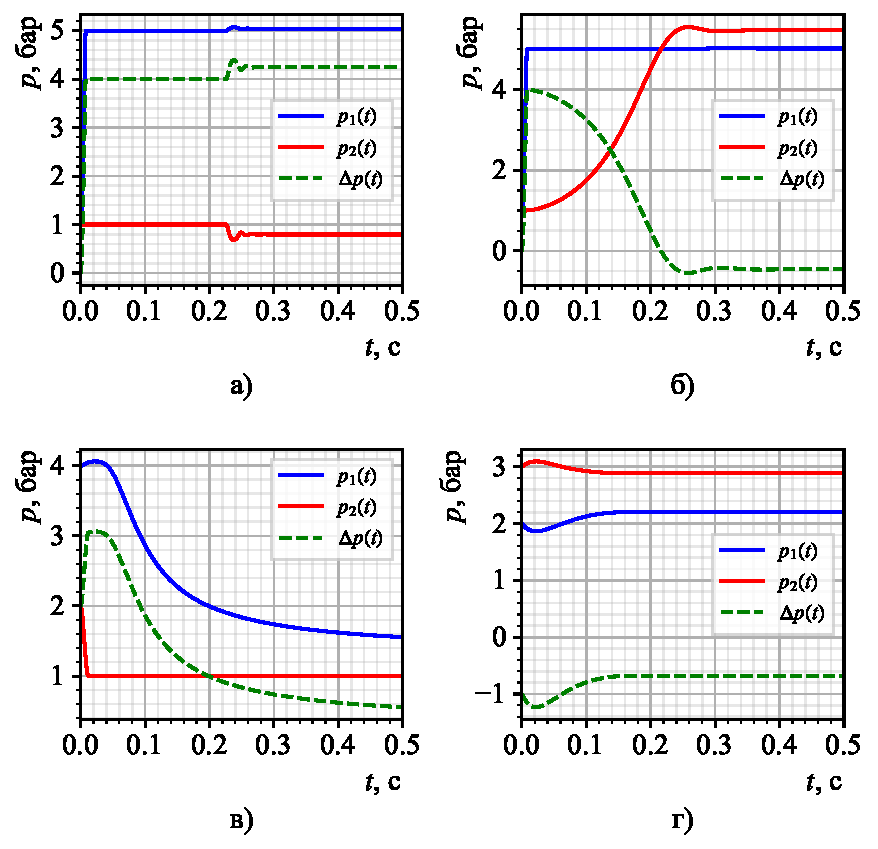
\includegraphics{part3/pressure_dynamics.pdf}
	\caption{Сравнение динамики установления давлений в различных режимах работы:\\
		а) сильное ускорение; б) умеренное ускорение; в) слабое ускорение; г) режим удержания}
	\label{fig:pressure_comparison}
\end{figure}

Представленные характеристик показывает существенное различие в динамике установления давлений для разных режимов работы.

В режиме сильного положительного ускорения [1,0,0,1] наблюдается максимальный
перепад давлений между полостями цилиндра, что подтверждается системой уравнений:

$$\begin{cases}
		\dot{p}_1 = \frac{\gamma RT_1}{V_1(x)}(G_{1,max} - \frac{p_1}{RT_1}F_1\dot{x}) \\
		\dot{p}_2 = \frac{\gamma RT_2}{V_2(x)}(-G_{4,max} + \frac{p_2}{RT_2}F_2\dot{x})
	\end{cases}$$
где $G_{1,max}$ и $G_{4,max}$ -- максимальные массовые расходы через соответствующие распределители.

Характерной особенностью данного режима является быстрый рост давления $p_1$ до величины, близкой к давлению питания
$p_\text{п}$, с одновременным падением давления $p_2$ до атмосферного давления $p_\text{атм}$. Это обеспечивает интенсивный
разгон штока с последующим выходом на установившуюся скорость, что наглядно демонстрируется на
фазовом портрете (рис. \ref{fig:pp_strong_accelration}). Анализ фазового портрета показывает,
что процесс выхода на установившуюся скорость характеризуется движением изображающей
точки по траектории, асимптотически стремящейся к прямой $v = v_\text{уст}$.

\begin{figure}[htbp]
	\centerfloat{
		\hfill
		\subcaptionbox[List-of-Figures entry]{\label{fig:pp_strong_acceleration_positive}}{
			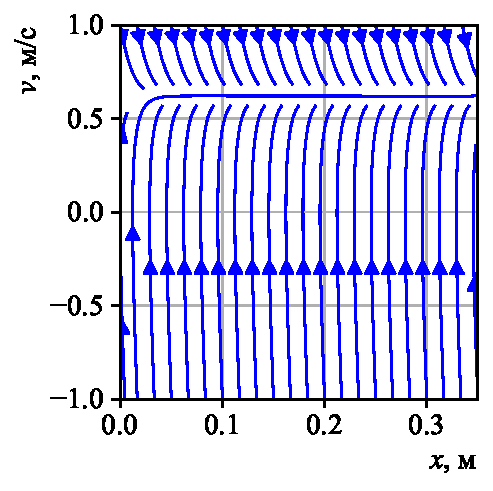
\includegraphics{part3/pp_strong_acceleration_positive.pdf} }
		\hfill
		\subcaptionbox{\label{fig:pp_strong_acceleration_negative}}{
			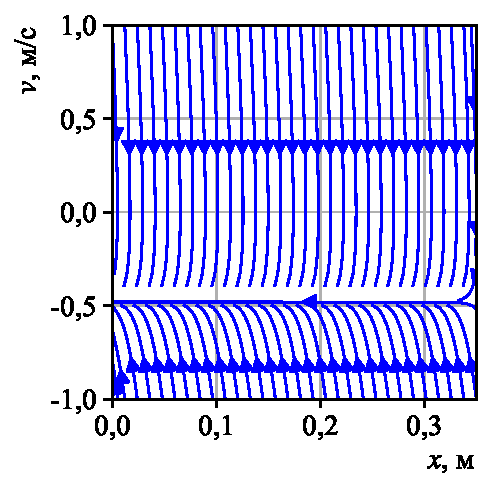
\includegraphics{part3/pp_strong_acceleration_negative.pdf} }
	}
	\caption{Фазовые портреты для режима сильного ускорения:\\
		а) положительное ускорение; б) отрицательное ускорение}
	\label{fig:pp_strong_accelration}
\end{figure}

В режимах умеренного ускорения [1,0,0,0]
наблюдается более сложная динамика, обусловленная асимметричным изменением давлений.
При данном режиме динамика давлений описывается системой:

\begin{equation*}
	\begin{cases}
		\dot{p}_1 = \frac{\gamma RT_1}{V_1(x)}(G_{1,max} - \frac{p_1}{RT_1}F_1\dot{x}) \\
		\dot{p}_2 = -\frac{\gamma p_2}{V_2(x)}F_2\dot{x}
	\end{cases}
\end{equation*}

Особенность данного режима заключается в том, что давление в штоковой полости изменяется согласно политропному процессу:

\begin{equation*}
	p_2V_2(x)^n = p_{2,0}V_{2,0}^n = \text{const}
\end{equation*}
где $p_{2,0}$ и $V_{2,0}$ -- начальное давление и объем штоковой полости соответственно в момент запирания полости;
$n$ - показатель политропы.

На фазовых портретах представленных на рисунке \ref{fig:pp_moderate_position_1} и рисунке \ref{fig:pp_moderate_position_2}
отчетливо видно влияние начальных условий на динамику системы. При большем начальном положении штока ($x_0$ равное 0,2~\si{\metre}) наблюдается более
интенсивное торможение вследствие меньшего начального объема запертой полости и, соответственно, более быстрого роста давления при сжатии воздуха.

\begin{figure}[htbp]
	\centerfloat{
		\hfill
		\subcaptionbox[List-of-Figures entry]{\label{fig:pp_medium_acceleration_x_01}}{
			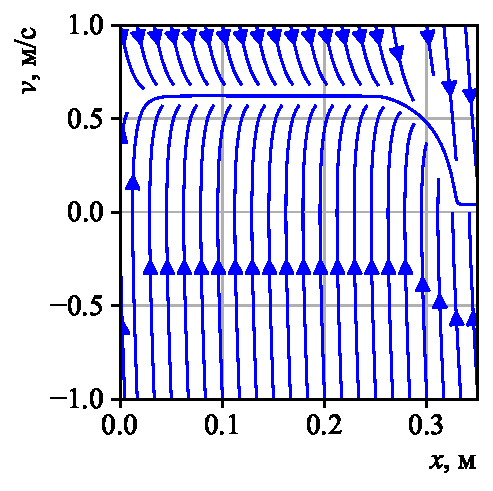
\includegraphics{part3/pp_medium_acceleration_x_01.pdf} }
		\hfill
		\subcaptionbox{\label{fig:pp_medium_acceleration_x_01_scheme}}{
			\raisebox{0.5\height}{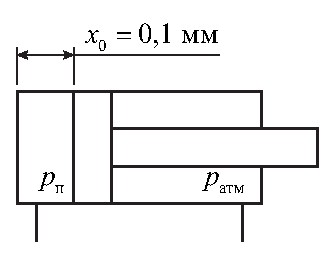
\includegraphics{part3/pp_medium_acceleration_x_01_scheme.eps}} }
	}
	\caption{Фазовый портрет и схема пневмоцилиндра при начальном положении штока $x_0 = \num{0.1}$ м ($p_{2,0} = p_\text{атм}$):\\
		а) фазовый портрет; б) схема пневмоцилиндра}
	\label{fig:pp_moderate_position_1}
\end{figure}

\begin{figure}[htbp]
	\centerfloat{
		\hfill
		\subcaptionbox[List-of-Figures entry]{\label{fig:pp_medium_acceleration_x_02}}{
			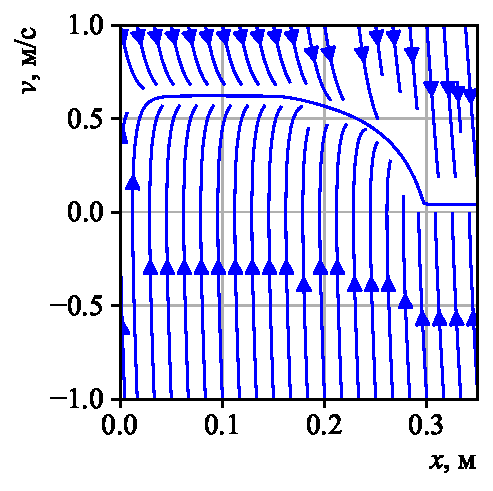
\includegraphics{part3/pp_medium_acceleration_x_02.pdf} }
		\hfill
		\subcaptionbox{\label{fig:pp_medium_acceleration_x_02_scheme}}{
			\raisebox{0.5\height}{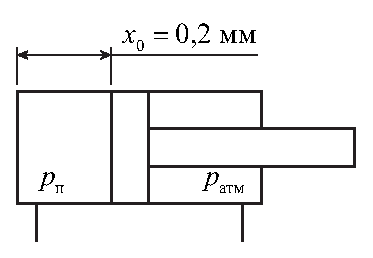
\includegraphics{part3/pp_medium_acceleration_x_02_scheme.eps}} }
	}
	\caption{Фазовый портрет и схема пневмоцилиндра при начальном положении штока $x_0 = \num{0.2}$ м ($p_{2,0} = p_\text{атм}$):\\
		а) фазовый портрет; б) схема пневмоцилиндра}
	\label{fig:pp_moderate_position_2}
\end{figure}

Для более полного понимания влияния начальных условий на динамику системы рассмотрена серия фазовых
портретов при различных комбинациях начального положения штока и давления в запираемой
полости (рис. \ref{fig:pp_moderate_matrix}). Анализ данных портретов демонстрирует, что при
фиксированном начальном положении увеличение давления $p_{2,0}$ приводит к снижению установившейся скорости
движения и увеличению интенсивности торможения. При фиксированном начальном давлении
увеличение координаты $x_0$ вызывает сокращение области достижимых состояний и смещение точки остановки к начальному положению.

\begin{figure}[htbp]
	\centerfloat{
		\hfill
		\subcaptionbox[List-of-Figures entry]{\label{fig:pp_medium_acceleration_x_01_p_2}}{
			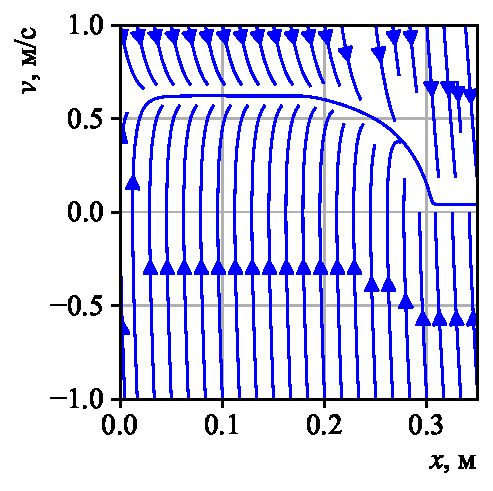
\includegraphics{part3/pp_medium_acceleration_x_01_p_2.pdf} }
		\hfill
		\subcaptionbox{\label{fig:pp_medium_acceleration_x_01_p_4}}{
			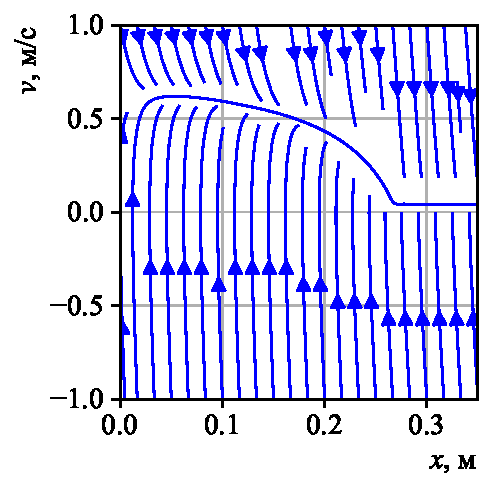
\includegraphics{part3/pp_medium_acceleration_x_01_p_4.pdf}}
		\hfill
		\subcaptionbox{\label{fig:pp_medium_acceleration_x_02_p_2}}{
			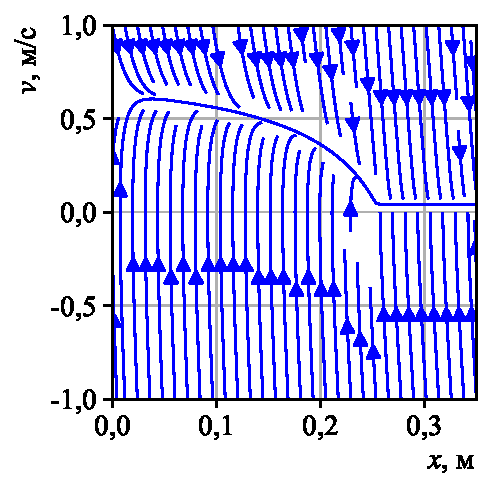
\includegraphics{part3/pp_medium_acceleration_x_02_p_2.pdf}}
		\hfill
		\subcaptionbox{\label{fig:pp_medium_acceleration_x_02_p_3}}{
			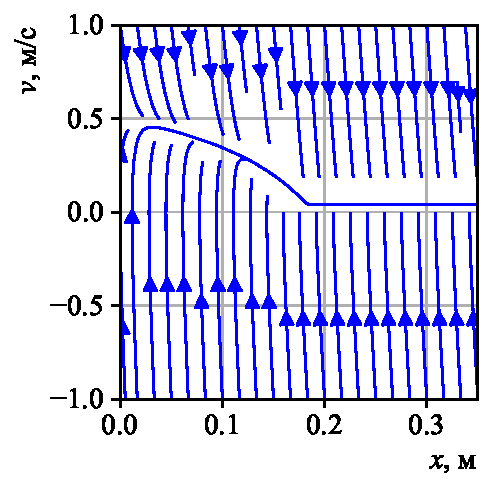
\includegraphics{part3/pp_medium_acceleration_x_02_p_4.pdf}}
	}
	\caption{Фазовые портреты при различных начальных условиях: \\
		а) $x_0 = \num{0,1}$ м, $p_{2,0} = 2$ бар; б) $x_0 = \num{0.1}$ м, $p_{2,0} = 4$ бар; \\
		в) $x_0 = \num{0.2}$ м, $p_{2,0} = 2$ бар; г) $x_0 = \num{0.2}$ м, $p_{2,0} = 4$ бар;
	}
	\label{fig:pp_moderate_matrix}
\end{figure}

Математически наблюдаемые эффекты описываются уравнением баланса сил:

\begin{equation*}
	p_\text{п}F_1 - p_{2,0}\left(\frac{V_{2,0}}{V_2(x)}\right)^nF_2 = R_\text{тр}(v),
\end{equation*}
где $V_2(x) = V_{2,0} + A_2(L - x)$ -- текущий объем запертой полости.

Режимы слабого ускорения [0,0,0,1] или [0,1,0,0] характеризуются минимальным перепадом давлений между
полостями пневмоцилиндра. Рассмотрим режим слабого положительного ускорения [0,0,0,1], при котором поршневая полость
изолирована, а штоковая соединена с атмосферой. Динамика давлений в данном режиме описывается системой уравнений:

$$\begin{cases}
		\dot{p}_1 = -\frac{\gamma p_1}{V_1(x)}F_1\dot{x} \\
		\dot{p}_2 = \frac{\gamma RT_2}{V_2(x)}(-G_{4,max} + \frac{p_2}{RT_2}F_2\dot{x})
	\end{cases}$$

На графиках отображенных на рисунке \ref{fig:pressure_comparison} видно, что давление $p_2$ снижается до
тмосферного значения существенно медленнее, чем в режиме сильного ускорения, в то время как
давление $p_1$ изменяется только за счет изменения объема поршневой полости. Данный процесс
характеризуется политропным изменением состояния воздуха в запертой полости:

\begin{equation*}
	p_1V_1(x)^n = p_{1,0}V_{1,0}^n = \text{const}
\end{equation*}
где $p_{1,0}$ и $V_{1,0}$ -- начальные значения давления и объема поршневой полости соответственно.

\begin{figure}[htbp]
	\centerfloat{
		\hfill
		\subcaptionbox[List-of-Figures entry]{\label{fig:pp_weak_acceleration_x01}}{
			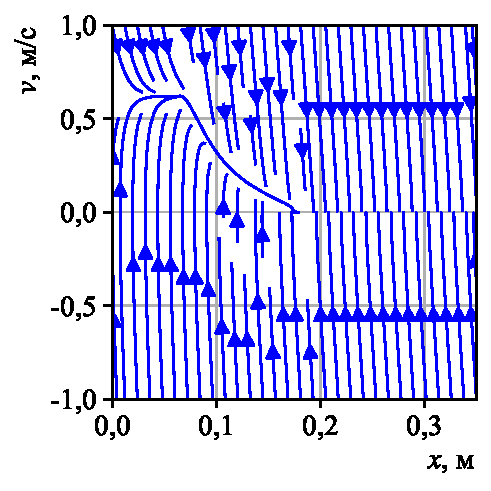
\includegraphics{part3/pp_slow_acceleration_x_01_p_3.pdf} }
		\hfill
		\subcaptionbox{\label{fig:pp_weak_acceleration_x02}}{
			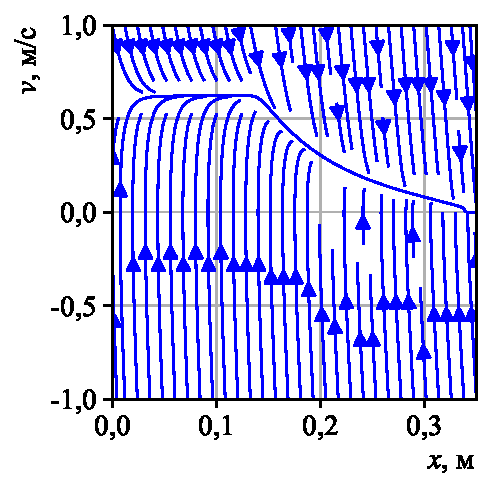
\includegraphics{part3/pp_slow_acceleration_x_02_p_3.pdf} }
	}
	\caption{Фазовые портреты для режима слабого ускорения при различных начальных условиях:\\
		а) $x_0 = \num{0.1}$ м, $p_{1,0} = 3$ бар; б) $x_0 = \num{0.2}$ м, $p_{1,0} = 3$ бар}
	\label{fig:pp_weak_acceleration}
\end{figure}

Анализ фазовых портретов представленных на рисунке \ref{fig:pp_weak_acceleration} показывает существенное влияние начального
положения штока на динамику системы. При увеличении начальной координаты $x_0$ наблюдается снижение максимально достижимой
скорости и уменьшение пути перемещения до точки остановки. Это объясняется более быстрым падением давления $p_1$ при расширении
воздуха в запертой полости большего начального объема.

Уравнение баланса сил для данного режима имеет вид:

\begin{equation*}
	p_{1,0}\left(\frac{V_{1,0}}{V_1(x)}\right)^nF_1 - p_\text{атм}F_2 = R_\text{тр}(v)
\end{equation*}

где $V_1(x) = V_{1,0} + A_1x$ - текущий объем поршневой полости.

Характерной особенностью режима слабого ускорения является существенная зависимость динамики
от сил трения. На фазовых портретах это проявляется в виде более крутых траекторий
торможения и меньшей области достижимых состояний по сравнению с режимами сильного и
умеренного ускорения. Данный эффект объясняется тем, что движущая сила, определяемая
разностью давлений в полостях, сопоставима по величине с силами трения.

Для оценки влияния начального давления в запертой полости на динамику системы рассмотрим
серию фазовых портретов при различных значениях $p_{1,0}$ приведенных на рисунке \ref{fig:pp_weak_pressure_matrix}.

\begin{figure}[htbp]
	\centerfloat{
		\hfill
		\subcaptionbox[List-of-Figures entry]{\label{fig:pp_weak_p2}}{
			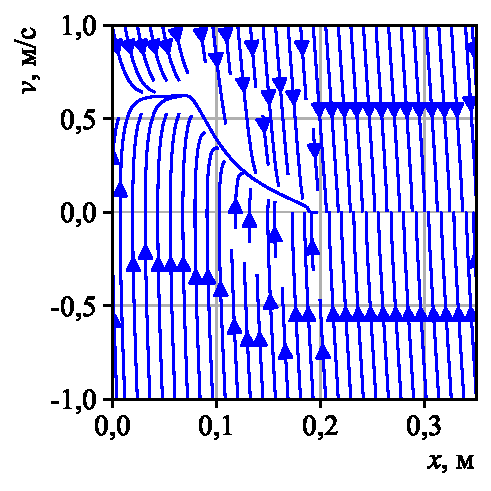
\includegraphics{part3/pp_slow_acceleration_x_015_p_2.pdf} }
		\hfill
		\subcaptionbox{\label{fig:pp_weak_p3}}{
			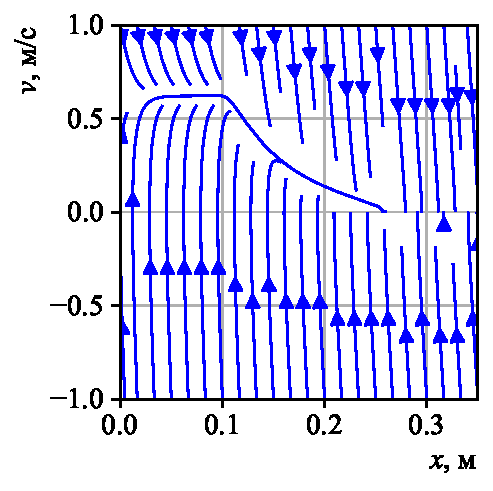
\includegraphics{part3/pp_slow_acceleration_x_015_p_3.pdf} }
		\vfill
		\subcaptionbox{\label{fig:pp_weak_p4}}{
			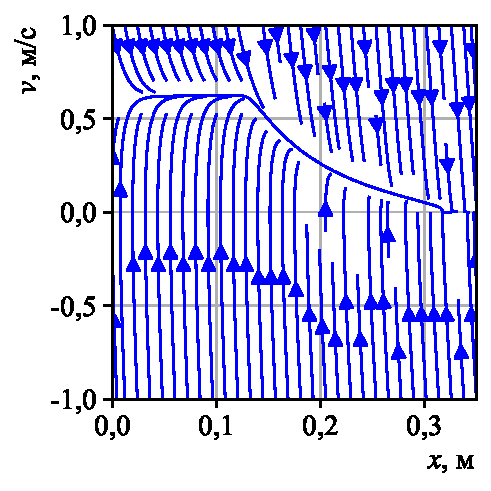
\includegraphics{part3/pp_slow_acceleration_x_015_p_4.pdf} }
	}
	\caption{Фазовые портреты при $x_0 = \num{0.15}$ м и различных начальных давлениях:\\
		а) $p_{1,0} = 2$ бар; б) $p_{1,0} = 3$ бар; в) $p_{1,0} = 4$ бар}
	\label{fig:pp_weak_pressure_matrix}
\end{figure}

Анализ представленных фазовых портретов демонстрирует, что увеличение начального давления $p_{1,0}$ приводит
к возрастанию максимальной скорости движения и увеличению дальности перемещения штока. При этом форма
фазовых траекторий становится более пологой, что свидетельствует о меньшем влиянии сил трения
на динамику системы. Данный эффект объясняется увеличением движущей силы при сохранении характера
её изменения в процессе движения.

%%%%%%%%%%%%%%%%%%%%%%%% mode 0

Режим удержания [0,0,0,0] представляет особый интерес с точки зрения
динамики электропневматического привода, поскольку в данном режиме обе полости
пневмоцилиндра оказываются изолированными.Изменение давлений при этом
происходит исключительно за счет изменения объемов полостей и описывается системой уравнений:

$$\begin{cases}
		\dot{p}_1 = -\frac{\gamma p_1}{V_1(x)}F_1\dot{x} \\
		\dot{p}_2 = -\frac{\gamma p_2}{V_2(x)}F_2\dot{x}
	\end{cases}$$

На графиках изменения давлений, согласно рисунку \ref{fig:pressure_comparison}, наблюдается характерное
политропное изменение состояния воздуха в обеих полостях, описываемое уравнениями:

\begin{equation*}
	\begin{cases}
		p_1V_1(x)^n = p_{1,0}V_{1,0}^n = \text{const} \\
		p_2V_2(x)^n = p_{2,0}V_{2,0}^n = \text{const}
	\end{cases}
\end{equation*}

где $p_{1,0}$, $V_{1,0}$ и $p_{2,0}$, $V_{2,0}$ -- начальные значения давлений и объемов поршневой и штоковой полостей соответственно.

Стабилизация положения штока в режиме удержания обеспечивается преимущественно силами трения, а также дополнительно
поддерживается пневматической жёсткостью, создаваемой сжатым воздухом в изолированных полостях. Баланс сил в данном режиме описывается уравнением:

\begin{equation*}
	p_1F_1 - p_2F_2 = R_\text{тр}(v)
\end{equation*}

\begin{figure}[htbp]
	\centerfloat{
		\hfill
		\subcaptionbox[List-of-Figures entry]{\label{fig:pp_hold_low_pressure}}{
			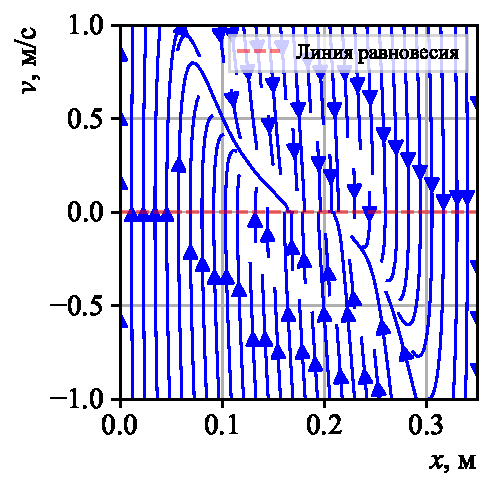
\includegraphics{part3/pp_hold_low_pressure.pdf} }
		\hfill
		\subcaptionbox{\label{fig:pp_hold_high_pressure}}{
			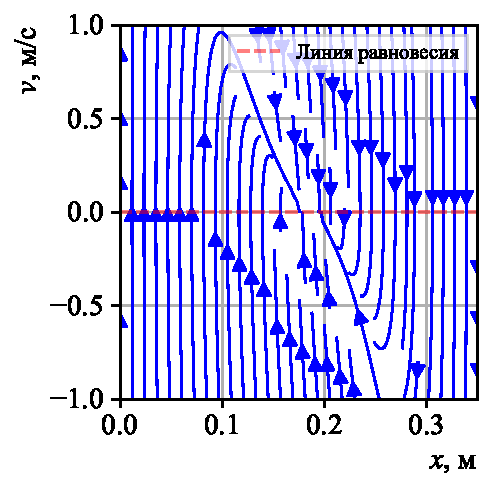
\includegraphics{part3/pp_hold_high_pressure.pdf} }
	}
	\caption{Фазовые портреты для режима удержания при различных начальных давлениях:\\
		а) низкие начальные давления ($p_{1,0} = 2$ бар, $p_{2,0} = \num{1.8}$ бар);\\
		б) высокие начальные давления ($p_{1,0} = 4$ бар, $p_{2,0} = \num{3.8}$ бар)}
	\label{fig:pp_hold_mode}
\end{figure}

Анализ фазовых портретов для режима удержания показанных на рисунке \ref{fig:pp_hold_mode} показывает высокую эффективность удержания положения штока при различных начальных давлениях.
В системе наблюдается апериодический характер движения с быстрым затуханием скорости, что обусловлено существенным влиянием сил трения.
При этом уровень начальных давлений в полостях оказывает незначительное влияние на характер переходного процесса, что подтверждается схожей формой фазовых траекторий.

\begin{figure}[htbp]
	\centerfloat{
		\hfill
		\subcaptionbox[List-of-Figures entry]{\label{fig:pp_hold_balanced}}{
			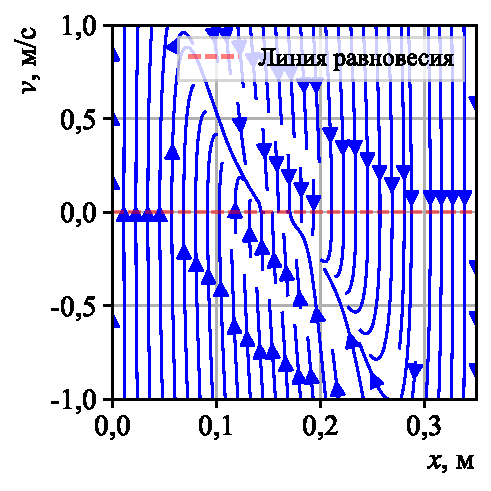
\includegraphics{part3/pp_hold_balanced.pdf} }
		\hfill
		\subcaptionbox{\label{fig:pp_hold_unbalanced}}{
			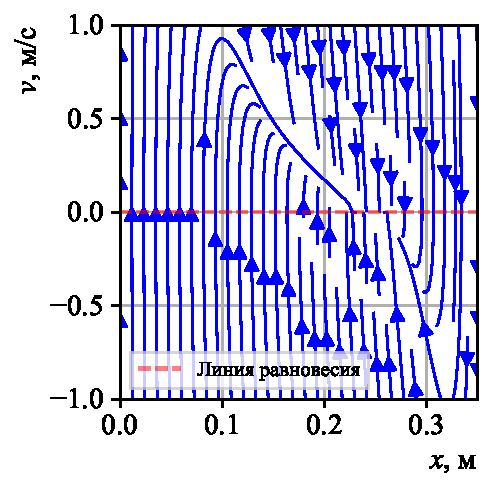
\includegraphics{part3/pp_hold_unbalanced.pdf} }
	}
	\caption{Фазовые портреты при $x_0 = \num{0.15}$ м и различных соотношениях начальных давлений:\\
		а) близкие давления ($p_{1,0} = 3$ бар, $p_{2,0} = 3$ бар);\\
		б) существенная разница ($p_{1,0} = 2$ бар, $p_{2,0} = 4$ бар)}
	\label{fig:pp_hold_matrix}
\end{figure}

Рассмотрение фазовых портретов при различных соотношениях начальных давлений отображенных на  рисунке \ref{fig:pp_hold_matrix} демонстрирует,
что даже при значительной разнице давлений в полостях система сохраняет устойчивое апериодическое движение к положению равновесия.
При близких значениях давлений $p_{1,0}$ и $p_{2,0}$ наблюдается симметричный характер фазовых траекторий. Увеличение разности давлений приводит к незначительной асимметрии траекторий при сохранении общего характера движения.

Математическое описание движения в окрестности положения равновесия может быть получено линеаризацией уравнений движения:

\begin{equation*}
	M\ddot{x} + \left(\frac{\gamma p_{1,0}F_1^2}{V_{1,0}} + \frac{\gamma p_{2,0}F_2^2}{V_{2,0}}\right)x + \nu\dot{x} = 0
\end{equation*}

где $\nu$ -- коэффициент вязкого трения. Существенное преобладание силы трения над пневматической жёсткостью
($\nu \gg \sqrt{M\left(\frac{\gamma p_{1,0}F_1^2}{V_{1,0}} + \frac{\gamma p_{2,0}F_2^2}{V_{2,0}}\right)}$) обуславливает апериодический характер движения системы.

Проведенный анализ режимов работы электропневматического привода с дискретными распределителями
позволил выявить характерные особенности динамики системы для каждого режима функционирования.
В режиме сильного ускорения [1,0,0,1] наблюдается максимальный перепад давлений между полостями и,
как следствие, наибольшая интенсивность разгона штока с последующим выходом на установившуюся скорость.
Режим умеренного ускорения [1,0,0,0] характеризуется существенным влиянием начальных условий на динамику
системы вследствие политропного изменения состояния воздуха в запертой полости. Режим слабого ускорения
[0,0,0,1] демонстрирует значительную зависимость от сил трения при минимальном перепаде давлений между полостями.
Особую роль играет режим удержания [0,0,0,0], в котором стабилизация положения штока обеспечивается преимущественно
силами трения при апериодическом характере затухания скорости. Построенные фазовые портреты и анализ динамики давлений
позволяют обоснованно подходить к выбору режимов работы при проектировании алгоритмов управления электропневматическим
приводом с дискретными распределителями. При этом учет выявленных закономерностей и особенностей каждого режима позволяет
обеспечить требуемые показатели качества позиционирования при минимизации количества переключений распределителей.

\section{ШИМ управление с использование ПИД регулятора}\label{sec:ch3/sec2}

\subsection{Принципы реализации ШИМ в пневматических системах с дискретным управлением}\label{subsec:ch3/sec2/sub1}
Широтно-импульсная модуляция (ШИМ) представляет собой метод формирования квазинепрерывного
управляющего воздействия в системах с дискретными исполнительными элементами.
В контексте пневматических систем с дискретными распределителями применение ШИМ
позволяет преодолеть ограничения, связанные с бинарным характером управления, и обеспечить более
точное регулирование положения и скорости исполнительного механизма.

Механизм формирования квазинепрерывного управляющего воздействия
посредством ШИМ основан на периодическом переключении дискретных
распределителей с определенной частотой и скважностью.

Математически это может быть описано следующим образом:

\begin{equation*}
	u(t) = \begin{cases}
		1, & 0 \leq t < \alpha T \\
		0, & \alpha T \leq t < T
	\end{cases}
\end{equation*}
где $u(t)$ -- управляющий сигнал;
$T$ -- период ШИМ;
$\alpha$ -- коэффициент заполнения $0 \leq \alpha \leq 1$.

На рисунке \ref{fig:ch3:pwm_example} показаны временные диаграммы ШИМ-сигнала
с различными значениями коэффициента заполнения.

\begin{figure}[ht]
	\centerfloat{
		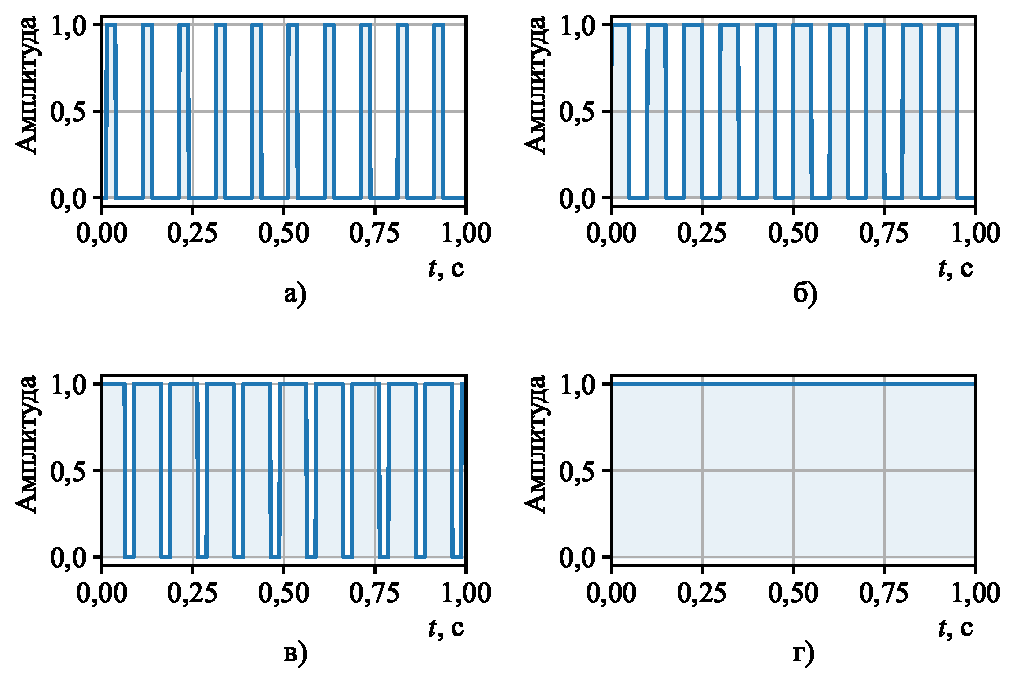
\includegraphics[]{part3/pwm_signal_skewness.pdf}
	}
	\caption{Примеры ШИМ-сигнала с различными значениями коэффициента заполнения:\\ а) $\alpha = \num{0.3}$; б) $\alpha = \num{0.6}$; в) $\alpha = \num{0.9}$}
	\label{fig:ch3:pwm_example}
\end{figure}

Среднее значение управляющего воздействия за период определяется как:
\begin{equation*}
	\bar{u} = \frac{1}{T} \int_0^T u(t) dt = \alpha,
\end{equation*}

Влияние частоты ШИМ на динамику пневмопривода является критическим фактором при
проектировании системы управления. С увеличением частоты ШИМ улучшается
гладкость управляющего воздействия, что способствует снижению пульсаций давления
и повышению точности позиционирования. Однако чрезмерно высокая частота может привести
к повышенному износу распределителей и увеличению энергопотребления.

Для анализа влияния частоты ШИМ на динамику системы может быть использована передаточная функция эквивалентного непрерывного звена:
\begin{equation*}
	W_{\text{ШИМ}}(s) = \frac{1 - e^{-sT}}{sT},
\end{equation*}
где $s$ -- комплексная переменная преобразования Лапласа.
Особенности применения ШИМ для различных типов дискретных
распределителей обусловлены их конструктивными характеристиками и
динамическими свойствами. На рисунке \ref{fig:ch3:pwm_valve_response} показаны
характеристики переходных процессов для распределителей с различным быстродействием.

\begin{figure}[ht]
	\centerfloat{
		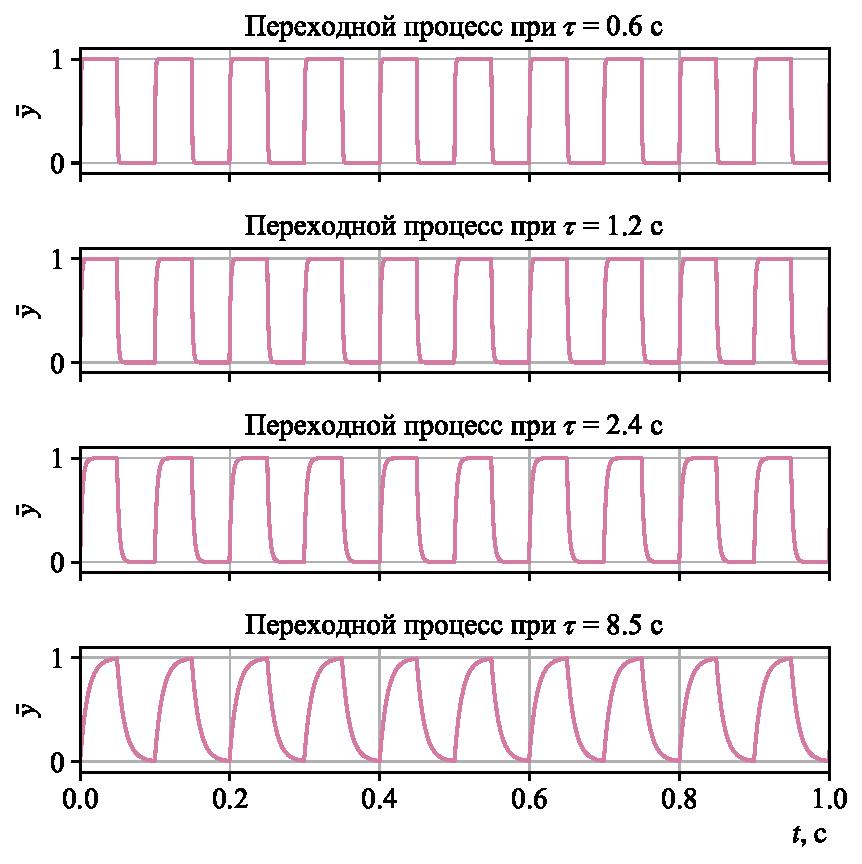
\includegraphics[]{part3/pwm_valve_response.pdf}
	}
	\caption{Характеристики переходных процессов для различных типов дискретных распределителей}
	\label{fig:ch3:pwm_valve_response}
\end{figure}

При выборе параметров ШИМ необходимо учитывать соотношение между
периодом ШИМ и динамическими характеристиками распределителя:
\begin{equation*}
	T_{ШИМ} \geq k\tau_{\text{р}},
\end{equation*}
где $\tau_{\text{р}}$ -- время реакции распределителя;
$k$ -- коэффициент запаса (обычно $k \geq 2$).

\subsection{Реализация ПИД-регулирования для пневмоприводов с дискретными распределителями}\label{subsec:ch3/sec2/sub2}
Применение ШИМ в пневмоприводах с дискретными распределителями открывает
возможность использования алгоритмов управления,
изначально разработанных для непрерывных систем.
Одним из наиболее эффективных и широко применяемых методов является
пропорционально-интегрально-дифференциальное (ПИД) регулирование.

Структура ПИД-регулятора для пневмопривода
с дискретными распределителями может быть представлена следующей схемой:
\begin{figure}[ht]
	\centerfloat{
		%    \includegraphics[]{part3/pid_pwn_control.pdf}
		\caption{Структурная схема ПИД-регулятора с ШИМ управлением}
	}
	\label{fig:ch3:pid_pwm_control}
\end{figure}
В данной схеме выходной сигнал ПИД-регулятора преобразуется в коэффициент
заполнения ШИМ, который управляет дискретными распределителями
пневмопривода. Этот подход позволяет достичь высокой точности
управления, характерной для непрерывных систем, в условиях
дискретного исполнительного механизма.

Математическая модель ПИД-регулятора в непрерывной форме описывается уравнением:
\begin{equation}\label{eq:pid_base}
	u_{\text{пид}}(t) = K_{\text{п}} e(t) + K_{\text{и}} \int_0^t e(\tau)d\tau + K_{\text{д}}\frac{de(t)}{dt},
\end{equation}
где
$e(t)$ -- ошибка регулирования;
$K_\text{п}$, $K_\text{и}$, $K_\text{д}$ -- коэффициенты пропорциональной, интегральной и
дифференциальной составляющих соответственно;

Выходной сигнал ПИД-регулятора преобразуется в коэффициент заполнения ШИМ согласно формуле:
\begin{equation*}
	\alpha = \frac{u(i) + u_{max}}{2u_{max}},
\end{equation*}
где $u_{max}$ -- максимальное значение управляющего сигнала.

Однако в рассматриваемой конфигурации ПП с дискретными распределителями
выходной сигнал ПИД-регулятора, как сказано выше, преобразутеся в бинарное
управляющее воздействие посредством ШИМ. При этом возможна только реализация
только двух основных режимов движения: выдвижение штока и его втягивание.

Математически это может быть описано следующим образом:

\begin{equation*}
	\mathbf{u}(t) = \begin{cases}
		[1,0,0,1], & \text{если } u_\text{пид}(t) > 0 \\
		[0,1,1,0], & \text{если } u_\text{пид}(t) < 0
	\end{cases}
\end{equation*}
где $u_\text{пид}(t)$ -- выходной сигнал ПИД-регулятора.

Существенным ограничением данного подхода является отсутствие
прямого управления режимом торможения привода, что может приводить к
перерегулированию и колебательности системы. Выходной сигнал ПИД-регулятора
преобразуется в коэффициент заполнения ШИМ согласно формуле:

\begin{equation*}
	\alpha = \begin{cases}
		\frac{u_\text{ПИД}(t)}{u_{max}},  & \text{если } u_\text{ПИД}(t) > 0 \\
		-\frac{u_\text{ПИД}(t)}{u_{max}}, & \text{если } u_\text{ПИД}(t) < 0
	\end{cases}
\end{equation*}
где $u_{max}$ -- максимальное значение управляющего сигнала.

Данное ограничение является одной из ключевых причин для рассмотрения модифицированных
структур управления, способных обеспечить более эффективное торможение и позиционирование
привода за счет использования дополнительных режимов работы распределителей или реализации
торможения.

\subsection{Модифицированная структура ПИД-регулятора}\label{subsec:ch3/sec2/sub3}

Как было написано выше классическая структура ПИД-регулятора с ШИМ управлением имеет существенные ограничения
в обеспечении эффективного управления электропневматическим приводом с дискретными распределителями.
Основным недостатком является отсутствие прямого управления режимом торможения, что приводит к значительному
перерегулированию и колебательности системы. Для преодоления данных ограничений предлагается модифицированная
структура ПИД-регулятора, обеспечивающая адаптивное торможение на основе анализа динамического состояния системы.

Предложенная модификация базируется на концепции прогнозирования тормозного пути и формировании упреждающего
управляющего воздействия. Математическая модель модифицированного ПИД-регулятора включает три основных
компонента: классический ПИД-регулятор описанный выражением \ref{eq:pid_base}, блок прогнозирования тормозного пути
и блок формирования тормозного воздействия.

Прогнозирование тормозного пути осуществляется на основе анализа
кинетической энергии системы и желаемого ускорения торможения:
\begin{equation*}\label{eq:braking_prediction}
	s_{\text{торм}}(t) = \frac{v(t)|v(t)|}{2a_{\text{торм}}} + \frac{K_{\text{б}}v(t)^2}{2},
\end{equation*}
где $v(t)$ -- текущая скорость привода;
$a_{\text{торм}}$ -- желаемое ускорение торможения;
$K_{\text{б}}$ -- коэффициент запаса по тормозному пути, учитывающий инерционность пневматической системы.

Эффективность торможения определяется соотношением между прогнозируемым тормозным путем
и расстоянием до целевой точки. Коэффициент интенсивности торможения вычисляется с использованием нелинейной функции:
\begin{equation*}\label{eq:braking_intensity_expanded}
	k_{\text{торм}}(t) = \begin{cases}
		\left(1 - \min\left(\frac{s_{\text{цель}}(t)}{s_{\text{торм}}(t) \cdot k_{\text{порог}}}, 1\right)\right)^2 \cdot \eta(v), & |v(t)| > v_{\text{порог}}    \\
		0,                                                                                                                         & |v(t)| \leq v_{\text{порог}}
	\end{cases}
\end{equation*}
где $s_{\text{цель}}(t) = |x_{\text{зад}} - x(t)|$ -- расстояние до целевой точки;
$k_{\text{порог}}$ -- пороговый коэффициент начала торможения;
$\eta(v)$ -- функция модуляции интенсивности торможения:
\begin{equation*}\label{eq:modulation_function}
	\eta(v) = 1 - \exp\left(-\left(\frac{|v(t)|}{v_{\text{хар}}}\right)^2\right),
\end{equation*}
где $v_{\text{хар}}$ -- характерная скорость, определяющая форму функции модуляции.

Результирующее управляющее воздействие формируется путем комбинации сигналов ПИД-регулятора и тормозного контура:
\begin{equation*}\label{eq:combined_control}
	u_{\text{м}}(t) = (1 - k_{\text{торм}}(t))u_{\text{пид}}(t) + k_{\text{торм}}(t)u_{\text{торм}}(t),
\end{equation*}
где $u_{\text{торм}}(t)$ -- сигнал управления в режиме торможения, определяемый направлением движения:
\begin{equation*}\label{eq:braking_control_expanded}
	\mathbf{u}_{\text{торм}}(t) = \begin{cases}
		[0, \alpha{\text{т}}(t), \alpha_{\text{т}}(t), 0],  & v(t) > v_{\text{порог}}      \\
		[\alpha_{\text{т}}(t), 0, 0, \alpha_{\text{т}}(t)], & v(t) < -v_{\text{порог}}     \\
		[0, 0, 0, 0],                                       & |v(t)| \leq v_{\text{порог}}
	\end{cases}
\end{equation*}

Коэффициент заполнения ШИМ в режиме торможения вычисляется с учетом динамических характеристик системы:
\begin{equation*}\label{eq:braking_pwm_expanded}
	\alpha_{\text{т}}(t) = k_{\text{торм}}(t) \cdot \alpha_{\text{макс}} \cdot \left(1 + K_{\text{к}}\frac{d|v(t)|}{dt}\right),
\end{equation*}
где $K_{\text{к}}$ -- коэффициент коррекции, учитывающий скорость изменения модуля скорости.

Для обеспечения численной устойчивости и плавности переключения режимов вводится гистерезисная характеристика активации торможения:
\begin{equation*}\label{eq:hysteresis}
	v_{\text{порог}}(t) = v_{\text{порог}}^0 \cdot \begin{cases}
		1 + \Delta v, & \text{при переходе к торможению} \\
		1 - \Delta v, & \text{при выходе из торможения}
	\end{cases}
\end{equation*}
где $v_{\text{порог}}^0$ -- базовое пороговое значение скорости;
$\Delta v$ -- ширина гистерезиса.

Исследование динамических характеристик системы управления электропневматическим приводом демонстрирует существенные различия
в характере переходных процессов для классической и модифицированной структур ПИД-регулятора с ШИМ.

Для классической структуры характерно наличие значительной колебательности, обусловленной отсутствием эффективного
управления торможением. Это проявляется в перерегулировании при подходе к заданной позиции и возникновении
затухающих колебаний из-за ограниченности режимов работы распределителей.

Модифицированная структура обеспечивает более качественный переходный процесс благодаря
адаптивному торможению и прогнозированию тормозного пути.

\begin{figure}[ht]
	\centerfloat{
		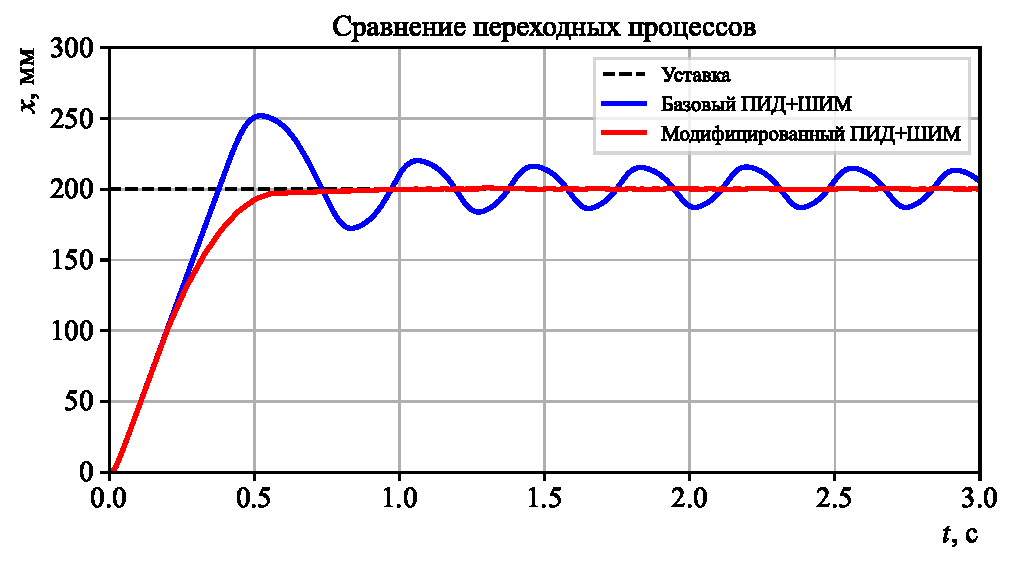
\includegraphics[]{part3/pid_comparison.pdf}
	}
	\caption{Сравнение переходных процессов для классической и модифицированной структуры ПИД-регулятора с ШИМ}
	\label{fig:ch3:transient_comparison}
\end{figure}

Представленные на рисунке \ref{fig:ch3:transient_comparison} результаты наглядно демонстрируют
преимущества модифицированной структуры в обеспечении качества позиционирования электропневматического привода.

% \subsection{Анализ динамических характеристик}\label{subsec:ch3/sec1/sub6}

\section{Управление в скользящих режимах}\label{sec:ch3/sec3}

\subsection{Теоретические основы многорежимного управления в скользящих режимах}\label{subsec:ch3/sec3/sub1}

Метод управления в скользящих режимах представляет собой робастный подход к управлению нелинейными системами, основанный на переключении структуры управления для обеспечения движения изображающей точки системы вдоль заданной поверхности скольжения в пространстве состояний. Рассмотрим теоретические основы данного метода применительно к задаче управления электропневматическим приводом с дискретными распределителями.

\subsection{Синтез алгоритмов управления в скользящих режимах}\label{subsec:ch3/sec3/sub2}



\section{Нечеткое управление}\label{sec:ch3/sec4}

\section{Прогнозное управление}\label{sec:ch3/sec5}
